In this section, the numerical results of the proposed UQ framework for the illustrative example in \sref{illustrative-example} are reported.\footnote{All the experiments are implemented in MATLAB R2012b \cite{matlab} and conducted on a GNU/Linux machine with Intel Core i7 3.4~GHz and 8~GB of RAM.}

The channel length $\Leff$ is assumed to deviate by $5\%$ from the nominal value of 45 nm where the global and local variations are equally weighted \cite{juan2011, juan2012}. The \rvs\ that represent the intra-die variability are computed by the KL expansion applied to \eref{covariance-function}; the procedure is described in \aref{uncertain-parameters} in the appendix. Dynamic power profiles involved in the experiments are based on simulations of randomly generated applications defined as directed acyclic task graphs.\footnote{The task graphs of the applications, floorplans of the platforms, configuration of HotSpot, which is used to construct the thermal RC circuits, are available online at \cite{sources}.} The floorplans of the platforms are constructed in such a way that the processing elements form regular grids, as it is the case with, \eg, Alpha 21264 studied in \cite{juan2011}. Time steps of power and temperature traces are set to one millisecond, \ie, $\dt_i = 10^{-3}$~s (see \sref{problem-formulation}). The reference leakage current $I_\leak(\Leff, \T)$ (see \sref{ie-power-model}) is scaled up to make the leakage power account for about $40\%$ of the total power at high temperatures \cite{liu2007}. To assess the performance of our framework, we employ a Monte Carlo (MC) sampling technique. For each sample, \ie, for each outcome of the uncertain parameters, the MC approach solves the initial problem numerically using the Dormand-Prince (DP) method provided by MATLAB; the procedure combines the well-known fourth- and fifth-order Runge-Kutta formulae \cite{press2007}. Based on theoretical estimates \cite{diaz-emparanza2002} of the accuracy of MC, experience from the literature \cite{xiu2010, eldred2009, maitre2010, shen2009}, and our observations, we let the MC approach with $10^4$ samples be the etalon for the evaluation of the proposed UQ framework.

\begin{figure}
  \centering
  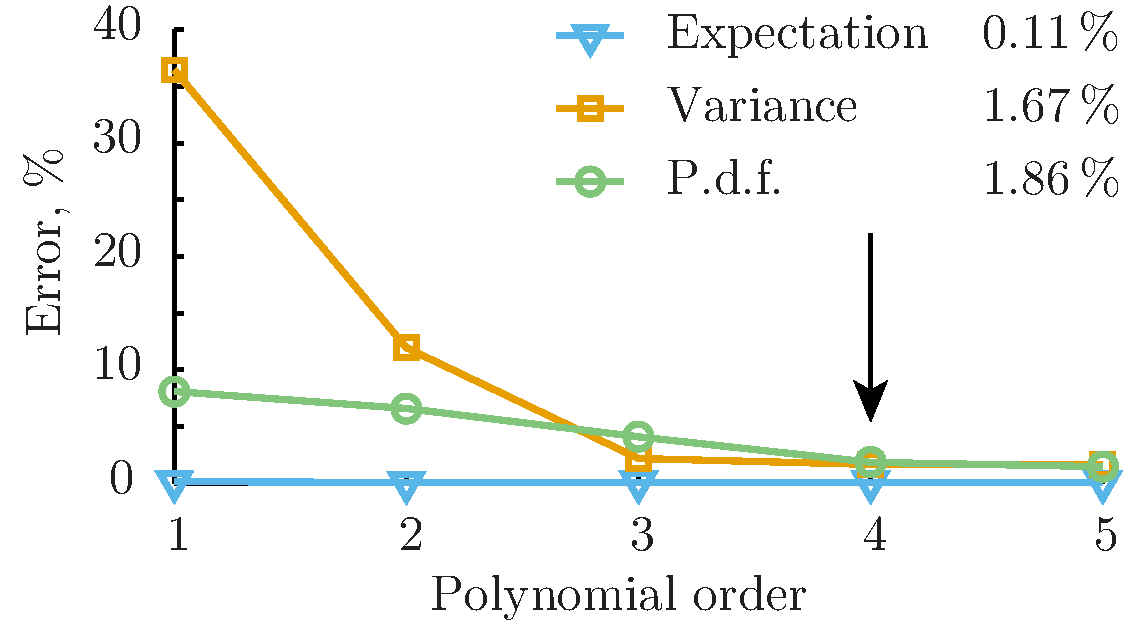
\includegraphics[width=1.0\columnwidth]{include/assets/accuracy.pdf}
  \caption{Errors of expectation, variance, and \pdf}
  \flabel{accuracy}
  \vspace{-1.6em}
\end{figure}

The first set of experiments is aimed to identify the accuracy of our technique and, consequently, to find a reasonable value of the polynomial order $\pcorder$ (see \sref{polynomial-chaos}). To this end, three accuracy metrics have been chosen. The first two are the normalized root-mean-square errors (\nrmse) of expectation and variance of the resulting temperature traces. The third metric is the mean of \nrmses\ of empirical \pdfs\ constructed at each time step for each processing element. The comparison for a quad-core architecture with a dynamic power profile of $\steps = 10^2$ steps is given in \fref{accuracy}, where $\pcorder$ is swept from one to six. It can be seen that the deviation of expectation is relatively small even for $\pcorder = 1$ and is bounded by $1\%$. The \nrmse\ of variance starts from $36\%$ for the first-order PC expansion and drops significantly to less than $2\%$ for the fifth-order PC. The result of the third error estimate, the \nrmse\ of \pdfs, is of particular importance since it allows us to conclude that the \pdfs\ computed by the fifth-order (and higher) PC are closely following those of the MC technique with a large number of samples. Guided by the above observations, we fix the polynomial order $\pcorder$ to five for the rest of the experiments and conclude that the error of our technique is bounded by less than $0.5\%$ for expectation and less than $2\%$ for variance and \pdf

\begin{table}[b]
  \vspace{-16pt}
  \centering
  \caption{Scaling with the number of processing elements $\cores$.}
  \begin{tabular*}{0.85\linewidth}{p{20pt}crrr}
    \toprule
    $\cores$ & $\vars$ & PC, seconds & MC, hours & Speedup, times \\
    \midrule
    $ 2$ & $2$ & $ 0.32$ & $31.24$ & $3.55 \times 10^5$ \\
    $ 4$ & $3$ & $ 0.45$ & $30.88$ & $2.46 \times 10^5$ \\
    $ 8$ & $4$ & $ 1.26$ & $31.44$ & $9.01 \times 10^4$ \\
    $16$ & $5$ & $ 6.55$ & $38.34$ & $2.11 \times 10^4$ \\
    $32$ & $6$ & $40.29$ & $41.58$ & $3.72 \times 10^3$ \\
    \bottomrule
  \end{tabular*}
  \tlabel{scaling-cores}
  \vspace{5pt}
  \caption{Scaling with the number of steps $\steps$.}
  \begin{tabular*}{0.85\linewidth}{p{42pt}rrr}
    \toprule
    $\steps$ & PC, seconds & MC, hours & Speedup, times \\
    \midrule
    $   10$ & $ 0.04$ & $   0.88$ & $8.19 \times 10^4$ \\
    $ 10^2$ & $ 0.06$ & $   3.12$ & $1.99 \times 10^5$ \\
    $ 10^3$ & $ 0.43$ & $  31.35$ & $2.65 \times 10^5$ \\
    $ 10^4$ & $ 4.35$ & $ 318.00$ & $2.63 \times 10^5$ \\
    $ 10^5$ & $42.23$ & $3110.29$ & $2.65 \times 10^5$ \\
    \bottomrule
  \end{tabular*}
  \tlabel{scaling-steps}
\end{table}

Now, we focus on the computational speed. In these experiments, we also provide results of a modified version of the MC sampling, in which the numerical solution via the DP method is replaced with the analytical solution described in \aref{thermal-model} and employed in \eref{recurrence}. First, we vary the number of processing elements $\cores$ while keeping the number of time steps $\steps$ constant and equal to $10^3$. The results are given in \tref{scaling-cores}, wherein the timing is in seconds, minutes, and hours for the proposed method (PM), analytical MC ($\text{MC}_\text{a}$), and numerical MC ($\text{MC}_\text{n}$), respectively. It can be seen that the proposed framework significantly outperforms the MC-based techniques. It is also apparent that our method benefits from both: the spectral decompositions, \ie, the PC and KL expansions, and the analytical solution used inside to tackle the thermal model. As an example, in order to quantify a power profile with $10^3$ steps of a multiprocessor system with 32 cores, the analytical and numerical MC approaches requires more than 15 minutes and 35 hours, respectively, whereas the proposed framework takes less than 10 seconds.

Finally, we investigate the scaling properties of the proposed UQ framework with respect to the number of time steps $\steps$ in the input dynamic power profile, which is directly proportional to the considered time span. The results for a quad-core architecture are given in \tref{scaling-steps}. Due to the long execution time demonstrated by the numerical MC approach, its computational times for high values of $\steps$ are extrapolated based on a smaller number of samples, \ie, $\mcsamples \ll 10^4$. It can be seen that all the methods scale linearly. However, the proposed framework shows a vastly superior performance.
